% ============================================================================
% gf-section.tex — drop-in section for paper.tex
% Place:  % ============================================================================
% gf-section.tex — drop-in section for paper.tex
% Place:  % ============================================================================
% gf-section.tex — drop-in section for paper.tex
% Place:  % ============================================================================
% gf-section.tex — drop-in section for paper.tex
% Place:  \input{gf-section}  immediately BEFORE  \section{The Fracture Gap
% and Defect Continuity}  (currently line ~702), so it follows the Asymptotic
% Penalty section whose coefficients it analyzes.
% Requires: figure at ../assets/out/delange-structure.pdf
%           (regenerate: scripts/gen_delange_figure.py)
% New bib entries: see references-additions.bib (trollope1968explicit,
% delange1975somme, allouche1992ring, allouche2003automatic,
% adamczewski2017problem, wilf2006generatingfunctionology).
% The generating-function/Mahler identities (Props ogf, mahler) and the
% closed-form/density decomposition are checked by
% scripts/verify_gf_identities.py for finitely many R (series to order 600;
% density decomposition for R < 2^16; closed forms over their scripted ranges).
% consistency check, not a proof: it does not (and cannot) establish the
% section's genuinely analytic claims — nowhere-differentiability in
% Theorem them:delange and transcendence in Corollary cor:transcend rest on
% their own arguments/citations; the supremum in Remark rem:extremal is not
% proven at all, and is presented there only as numerical evidence.
% ============================================================================

\section{Analytic Structure of the Boundary Coefficients}\label{sec:analytic}

The extraconnectivity formula~\eqref{eq:extraconnectivity} is governed by two
integer sequences: the cumulative binary weight $\Eseq(R)$ (OEIS A000788) and
the correction constant $\Cconst(R)$, linked by the closed
form~\eqref{eq:cconst}. In this section we place these coefficients in their
classical analytic context: we derive their ordinary generating functions in
the style of Wilf~\cite{wilf2006generatingfunctionology}, exhibit an exact
Mahler functional equation certifying that no linear-recurrence
(rational-generating-function) closed form for them can exist, and import the
Trollope--Delange theorem to give the exact asymptotics of the boundary
formula, including a continuous, nowhere-differentiable periodic fluctuation
that the correction density inherits. Everything in this section is an
unconditional statement about the integer sequences themselves; it does not
depend on Propositions~\ref{prop:universal} or~\ref{prop:hb-eval}. Via
Proposition~\ref{prop:hb-eval}, the difference $\Cconst(R) - \Eseq(R)$ acquires
its graph-theoretic reading as the cross-collision count $X(\mathrm{HB}_R)$,
and we use that notation for it below.

\subsection{Ordinary generating functions}

Write $s_2(i) = \mathrm{popcount}(i)$ for the binary digit sum, so
$\Eseq(R) = \sum_{i<R} s_2(i)$, and abbreviate the ceiling-log summand of
Definition~\ref{def:constants} by
$\lambda(i) = \lceil \log_2(i+1) \rceil$ (the bit length of $i$).

\begin{proposition}[Generating functions of the coefficients]\label{prop:ogf}
	As formal power series,
	\begin{align}
		\sum_{i \ge 0} s_2(i)\, x^i
		 & = \frac{1}{1-x} \sum_{j \ge 0} \frac{x^{2^j}}{1+x^{2^j}},
		\label{eq:ogf-s2}                                             \\
		\sum_{R \ge 0} \Eseq(R)\, x^R
		 & = \frac{x}{(1-x)^2} \sum_{j \ge 0} \frac{x^{2^j}}{1+x^{2^j}},
		\label{eq:ogf-E}                                              \\
		\sum_{R \ge 0} \Cconst(R)\, x^R
		 & = \frac{x^2}{(1-x)^2}
		+ \frac{x}{(1-x)^2} \sum_{j \ge 0} \frac{x^{2^{j+1}}}{1+x^{2^j}}.
		\label{eq:ogf-C}
	\end{align}
\end{proposition}

\begin{proof}
	The indicator of ``bit $j$ of $i$ is set'' is periodic in $i$ with period
	$2^{j+1}$ and pattern $0^{2^j} 1^{2^j}$; summing the geometric series over
	one period and over all periods gives
	$\sum_i [\,\text{bit } j \text{ of } i\,]\, x^i
		= x^{2^j} \frac{1-x^{2^j}}{1-x} \cdot \frac{1}{1-x^{2^{j+1}}}
		= \frac{x^{2^j}}{(1-x)(1+x^{2^j})}$.
	Summing over $j$ yields~\eqref{eq:ogf-s2} since
	$s_2 = \sum_j [\,\text{bit } j\,]$. Partial summation is multiplication by
	$x/(1-x)$: if $A(x) = \sum_i a_i x^i$ then
	$\sum_R \big(\sum_{i<R} a_i\big) x^R = \frac{x}{1-x} A(x)$, giving~\eqref{eq:ogf-E}.
	For~\eqref{eq:ogf-C}, the same period argument applied to the indicator
	$[\lambda(i) > j] = [i \ge 2^j]$ gives
	$\sum_i \lambda(i) x^i = \frac{1}{1-x}\sum_{j\ge0} x^{2^j}$, hence
	$\sum_R \big(\sum_{i<R}\lambda(i)\big) x^R = \frac{x}{(1-x)^2}\sum_j x^{2^j}$;
	combining with $\sum_{R \ge 1} (R-1)x^R = \frac{x^2}{(1-x)^2}$
	and~\eqref{eq:ogf-E} per Definition~\ref{def:constants}, the
	$\Eseq$-series cancels term-by-term against the $\lambda$-series via
	$\frac{x^{2^j}}{1} - \frac{x^{2^j}}{1+x^{2^j}} = \frac{x^{2^{j+1}}}{1+x^{2^j}}$.
\end{proof}

\subsection{A Mahler functional equation, and why no simpler closed form exists}

The radix-2 recurrences $\Eseq(2m) = 2\Eseq(m) + m$ and
$\Eseq(2m+1) = \Eseq(m) + \Eseq(m+1) + m$ that drive
Lemma~\ref{lem:subadditivity} translate, in the generating-function domain,
into a functional equation of Mahler type~--- the classical algebraic home of
divide-and-conquer sequences.

\begin{proposition}[Mahler equation]\label{prop:mahler}
	Let $S(x) = \sum_{i\ge0} s_2(i)x^i$ and $F(x) = \sum_R \Eseq(R) x^R$. Then
	\begin{equation}\label{eq:mahler}
		S(x) = (1+x)\, S(x^2) + \frac{x}{1-x^2},
		\qquad\text{equivalently}\qquad
		x\,F(x) = (1+x)^2\, F(x^2) + \frac{x^3}{(1-x)(1-x^2)} .
	\end{equation}
	In particular $S$ and $F$ are $2$-Mahler functions of order one, and
	$s_2$, $\Eseq$, and (via~\eqref{eq:cconst}) $\Cconst$ are $2$-regular
	sequences in the sense of
	Allouche--Shallit~\cite{allouche1992ring,allouche2003automatic}.
\end{proposition}

\begin{proof}
	Splitting $S$ over even and odd indices and applying
	$s_2(2m) = s_2(m)$, $s_2(2m+1) = s_2(m) + 1$ gives
	$S(x) = S(x^2) + x\,S(x^2) + x\sum_{m\ge0} x^{2m}$, which
	is~\eqref{eq:mahler}; the $F$-form follows from
	$F(x) = \frac{x}{1-x} S(x)$. Regularity of $s_2$ is the textbook example
	in~\cite{allouche1992ring}; the ring of $2$-regular sequences is closed
	under running sums (giving $\Eseq$). For $\Cconst$, write
	$d = \lceil \log_2 R \rceil$, the bit length of $R-1$ (for $R \ge 1$); it is a
	standard $2$-regular sequence~\cite{allouche1992ring}, as is
	$2^{d} = 2^{\lceil \log_2 R \rceil}$ (the round-up-to-a-power-of-$2$
	sequence), and $R$ is $2$-regular as a polynomial sequence; since the
	$2$-regular sequences form a ring (closed under both sums and products),
	$R(d{+}1) - 2^d$ is $2$-regular, and hence so is
	$\Cconst = R(d{+}1) - 2^d - \Eseq$ by~\eqref{eq:cconst}.
\end{proof}

The $2$-regular matrix representation is exactly what the characterization
engine exploits: \texttt{predict.cpp} evaluates $\Eseq(R)$ in $O(\log R)$ by
recursing on the binary expansion (Appendix~\ref{app:engine}), which is the
operational form of Proposition~\ref{prop:mahler}.

\begin{corollary}[No linear-recurrence closed form]\label{cor:transcend}
	$F(x)$ is transcendental over $\mathbb{Q}(x)$. Consequently $\Eseq(R)$
	(and hence $\Cconst(R)$) satisfies no linear recurrence with constant
	coefficients: the correction constants of
	Theorem~\ref{them:main} are not expressible by any rational generating
	function or polynomial-exponential closed form.
\end{corollary}

\begin{proof}
	We first show: no sequence of the form $a(R) = \tfrac{1}{2}R\log_2 R +
	O(R)$ is $C$-finite. Suppose $a(R) = \sum_i p_i(R)\lambda_i^R$ for
	finitely many algebraic $\lambda_i$ and polynomials $p_i$, not all zero.
	By Cauchy--Hadamard applied to the ordinary generating function of $a$,
	its radius of convergence is $1/\rho$ with $\rho = \max_i |\lambda_i|$,
	and $a(R)^{1/R} \to 1$ since $a(R) = \Theta(R\log R)$; hence $\rho = 1$,
	so every $|\lambda_i| \le 1$. Let $K \ge 0$ be the largest degree of
	$p_i$ among indices with $|\lambda_i| = 1$ (such indices exist, else
	$a(R) \to 0$), and let $h(R) = \sum_{|\lambda_i|=1} \mathrm{lead}(p_i)
	\lambda_i^R$ collect the corresponding leading coefficients; every other
	term is $o(R^K)$, so $a(R)/R^K - h(R) \to 0$. As $h$ is a nonzero finite
	sum of unit-modulus exponentials, orthogonality of distinct characters
	gives $\frac{1}{N}\sum_{R<N} |h(R)|^2 \to \sum_{|\lambda_i|=1}
	|\mathrm{lead}(p_i)|^2 > 0$, so $h$ is bounded (a finite trigonometric
	sum) but does not tend to $0$ in mean square; in particular $a(R)/R^K$
	is bounded and $\limsup_R |a(R)|/R^K > 0$. But $a(R)/R^K =
	\tfrac{1}{2}R^{1-K}\log_2 R + O(R^{1-K})$ tends to $\infty$ for $K \le 1$
	(contradicting boundedness) and to $0$ for $K \ge 2$ (contradicting
	positive limsup). No $K$ survives, so $a$ is not $C$-finite.

	Since $\Eseq(R) = \tfrac{1}{2}R\log_2 R + O(R)$ (Theorem~\ref{them:delange}
	below), $\Eseq$ is not $C$-finite by the above, so $F$ is not rational
	(a rational $F$ would make $\Eseq$ eventually satisfy a linear recurrence
	with constant coefficients, i.e.\ be $C$-finite). The identical growth
	class applies to $\Cconst$: writing $d = \lceil \log_2 R \rceil$,
	\eqref{eq:cconst} gives $\Cconst(R) = R(d{+}1) - 2^d - \Eseq(R)$, and
	since $2^{d-1} < R \le 2^d$ we have $2^d = \Theta(R)$, so
	$R(d{+}1) - 2^d = R\log_2 R + O(R)$; combined with the expansion of
	$\Eseq$ this gives $\Cconst(R) = \tfrac{1}{2}R\log_2 R + O(R)$, so
	$\Cconst$ is not $C$-finite either. A Mahler function that is algebraic
	over $\mathbb{Q}(x)$ is rational by the theorem of Adamczewski and
	Bell~\cite{adamczewski2017problem}; since $F$ satisfies~\eqref{eq:mahler}
	and is irrational, it is transcendental.
\end{proof}

\subsection{Exact asymptotics: the Trollope--Delange fluctuation}

\begin{theorem}[Trollope~\cite{trollope1968explicit};
		Delange~\cite{delange1975somme}]\label{them:delange}
	There is a continuous, nowhere-differentiable function
	$\Phi \colon \mathbb{R} \to \mathbb{R}$ of period $1$ such that for all
	$R \ge 1$,
	\begin{equation}\label{eq:delange}
		\Eseq(R) = \tfrac{1}{2} R \log_2 R + R\,\Phi(\log_2 R).
	\end{equation}
	The Fourier coefficients of $\Phi$ are known explicitly and involve the
	values of the Riemann zeta function at the points
	$2\pi i k/\log 2$ on the imaginary axis~\cite{delange1975somme}.
\end{theorem}

\begin{corollary}[Fluctuation of the correction densities]\label{cor:densities}
	Let $u = \{\log_2 R\}$ denote the fractional part and set
	$\Psi(u) = 2 - u - 2^{1-u}$. Then for all $R \ge 2$,
	\begin{align}
		\frac{\Cconst(R)}{R}
		 & = \tfrac{1}{2}\log_2 R \;+\; \Psi(u) \;-\; \Phi(\log_2 R),
		\label{eq:C-density}                                        \\
		\frac{X(\mathrm{HB}_R)}{R} \;=\; \frac{\Cconst(R)-\Eseq(R)}{R}
		 & = \Psi(u) \;-\; 2\,\Phi(\log_2 R).
		\label{eq:X-density}
	\end{align}
	In particular the cross-collision density
	$(\Cconst(R)-\Eseq(R))/R$ is a \emph{bounded}, purely oscillatory function
	of $\log_2 R$: it carries no growing term, vanishes exactly at the powers
	of two ($\Psi(0) = \Phi(d) = 0$), and is strictly positive elsewhere.
\end{corollary}

\begin{proof}
	Write $d = \lceil \log_2 R \rceil$, so for $R$ not a power of two
	$d = \log_2 R - u + 1$, and directly from the closed
	form~\eqref{eq:cconst},
	$\Cconst(R)/R = (d+1) - 2^d/R - \Eseq(R)/R
		= \log_2 R + (2 - u - 2^{1-u}) - \Eseq(R)/R$;
	substituting~\eqref{eq:delange} gives~\eqref{eq:C-density}, and
	subtracting $\Eseq(R)/R$ once more gives~\eqref{eq:X-density}. At
	$R = 2^d$ both sides agree in the limit $u \to 0^+$ and equal
	$\Cconst(2^d)/2^d - \tfrac{d}{2} = 0$, recovering
	$\Cconst(2^d) = \Eseq(2^d)$ and $X(\mathrm{HB}_{2^d}) = 0$. Boundedness
	of~\eqref{eq:X-density} follows since $\Psi$ and $\Phi$ are continuous and
	periodic; positivity away from powers of two is
	Proposition~\ref{prop:hb-eval}'s
	$X(\mathrm{HB}_R) = \Cconst(R) - \Eseq(R) \ge 0$ together with the strict
	inequality visible in the closed form.
\end{proof}

\begin{figure}[ht]
	\centering
	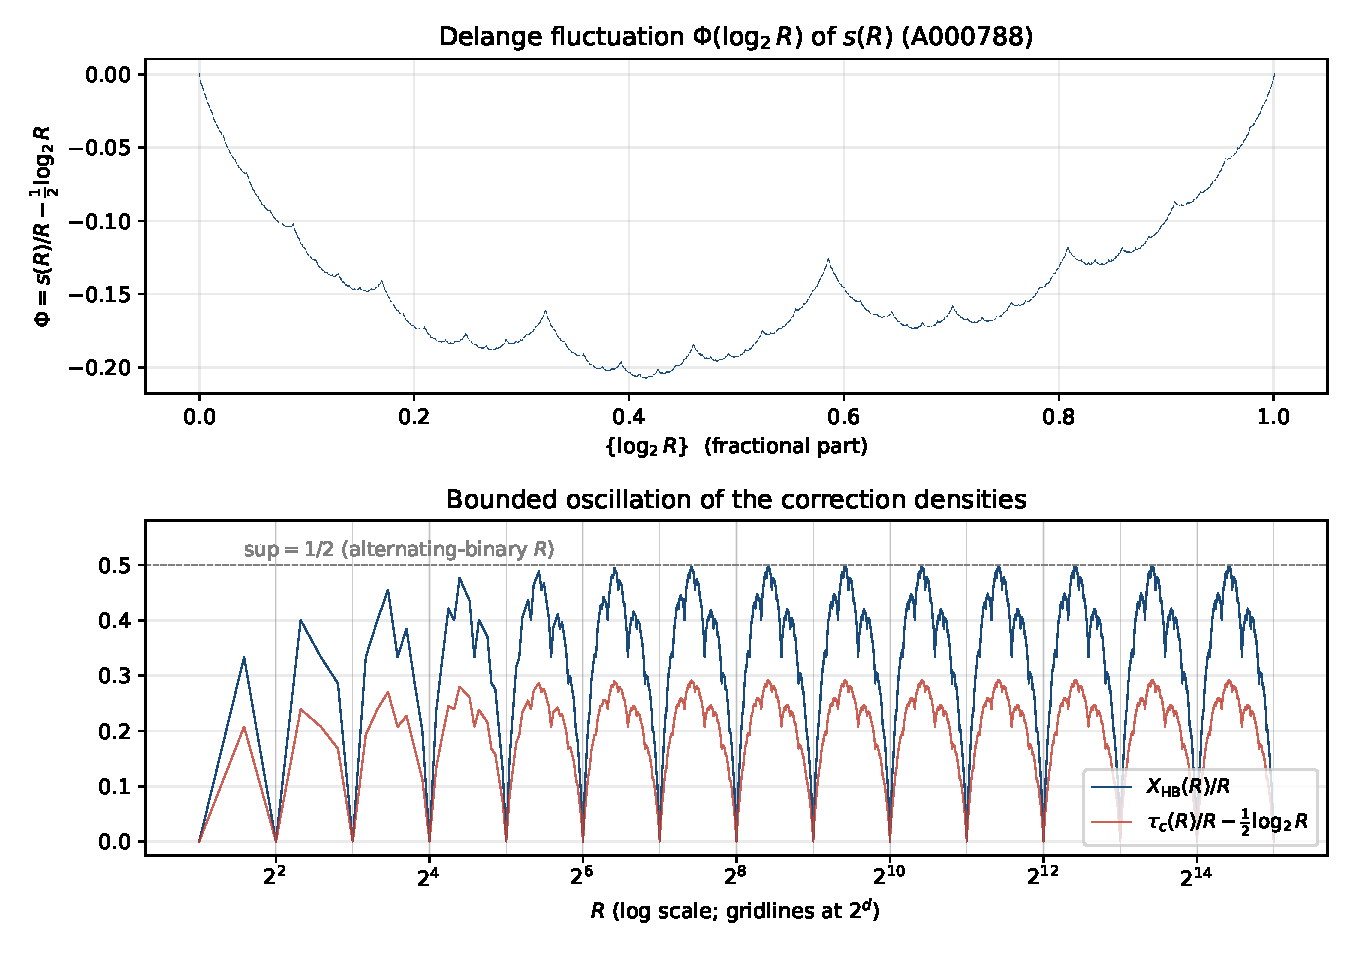
\includegraphics[width=0.92\textwidth]{../assets/out/delange-structure.pdf}
	\caption{Top: the Delange fluctuation $\Phi(\log_2 R)$
		of~\eqref{eq:delange}, computed from $\Eseq(R)$ for
		$256 \le R \le 2^{20}$ and plotted against $\{\log_2 R\}$; the
		self-similar, nowhere-differentiable profile is characteristic of
		radix-$2$ digital sums. Bottom: the centered correction density
		$\Cconst(R)/R - \tfrac{1}{2}\log_2 R$ and the cross-collision density
		$X(\mathrm{HB}_R)/R$ of Corollary~\ref{cor:densities} for
		$2 \le R \le 2^{15}$; both are bounded oscillations in $\log_2 R$,
		vanishing at every power of two (gridlines). The dashed line marks the
		empirical supremum $1/2$ of the cross-collision density, approached
		along the alternating-binary integers
		$R = \lceil 2^{d+1}/3 \rceil$ (e.g.\ $R = 43691 =
			(1010101010101011)_2$ attains $X/R > 0.49998$).}
	\label{fig:delange}
\end{figure}

\begin{remark}[Extremal densities]\label{rem:extremal}
	Numerically, $\sup_R X(\mathrm{HB}_R)/R = \tfrac{1}{2}$ for all sampled
	$R < 2^{16}$ (Figure~\ref{fig:delange}), approached along the
	alternating-binary integers $R = \lceil 2^{d+1}/3\rceil$, which are the
	classical extremizers of the Delange fluctuation; we record this as
	numerical evidence rather than a proven exact supremum, since we have
	not derived it from the Trollope--Delange expansion. The
	graph-theoretic reading is pleasing: the Hamming ball's shielding
	$4$-cycles appear, in this numerical range, to never exceed one per two
	vertices; the largest observed densities occur along the
	alternating-binary integers described above, and they disappear entirely when the ball
	closes into a full subcube.
\end{remark}

\begin{remark}[Relation to the Asymptotic Penalty]\label{rem:penalty-analogy}
	Corollary~\ref{cor:densities} quantifies exactly the $O_R(1)$ terms of
	Theorem~\ref{them:penalty}: in the boundary
	formula~\eqref{eq:extraconnectivity}, the dimension scaling contributes
	the exact linear term in $(n-k)$, while the correction density
	$\Cconst(R)/R$ splits, per~\eqref{eq:C-density}, into a logarithmic trend
	$\tfrac{1}{2}\log_2 R$ plus the bounded oscillation $\Psi(u) -
	\Phi(\log_2 R)$ that carries its entire remaining $R$-dependence.
	Readers
	familiar with analytic
	combinatorics~\cite{wilf2006generatingfunctionology} may recognize the
	division of labor: as in singularity analysis, where a dominant pole
	dictates growth and the remaining analytic part contributes bounded
	corrections, the identity of Theorem~\ref{them:penalty} separates the
	dominant $\Delta D \cdot (n-k)$ term from a topology-dependent constant
	--- though here the separation is an exact finite identity, proved
	directly in the discrete domain, rather than an asymptotic extraction.
\end{remark}
  immediately BEFORE  \section{The Fracture Gap
% and Defect Continuity}  (currently line ~702), so it follows the Asymptotic
% Penalty section whose coefficients it analyzes.
% Requires: figure at ../assets/out/delange-structure.pdf
%           (regenerate: scripts/gen_delange_figure.py)
% New bib entries: see references-additions.bib (trollope1968explicit,
% delange1975somme, allouche1992ring, allouche2003automatic,
% adamczewski2017problem, wilf2006generatingfunctionology).
% The generating-function/Mahler identities (Props ogf, mahler) and the
% closed-form/density decomposition are checked by
% scripts/verify_gf_identities.py for finitely many R (series to order 600;
% density decomposition for R < 2^16; closed forms over their scripted ranges).
% consistency check, not a proof: it does not (and cannot) establish the
% section's genuinely analytic claims — nowhere-differentiability in
% Theorem them:delange and transcendence in Corollary cor:transcend rest on
% their own arguments/citations; the supremum in Remark rem:extremal is not
% proven at all, and is presented there only as numerical evidence.
% ============================================================================

\section{Analytic Structure of the Boundary Coefficients}\label{sec:analytic}

The extraconnectivity formula~\eqref{eq:extraconnectivity} is governed by two
integer sequences: the cumulative binary weight $\Eseq(R)$ (OEIS A000788) and
the correction constant $\Cconst(R)$, linked by the closed
form~\eqref{eq:cconst}. In this section we place these coefficients in their
classical analytic context: we derive their ordinary generating functions in
the style of Wilf~\cite{wilf2006generatingfunctionology}, exhibit an exact
Mahler functional equation certifying that no linear-recurrence
(rational-generating-function) closed form for them can exist, and import the
Trollope--Delange theorem to give the exact asymptotics of the boundary
formula, including a continuous, nowhere-differentiable periodic fluctuation
that the correction density inherits. Everything in this section is an
unconditional statement about the integer sequences themselves; it does not
depend on Propositions~\ref{prop:universal} or~\ref{prop:hb-eval}. Via
Proposition~\ref{prop:hb-eval}, the difference $\Cconst(R) - \Eseq(R)$ acquires
its graph-theoretic reading as the cross-collision count $X(\mathrm{HB}_R)$,
and we use that notation for it below.

\subsection{Ordinary generating functions}

Write $s_2(i) = \mathrm{popcount}(i)$ for the binary digit sum, so
$\Eseq(R) = \sum_{i<R} s_2(i)$, and abbreviate the ceiling-log summand of
Definition~\ref{def:constants} by
$\lambda(i) = \lceil \log_2(i+1) \rceil$ (the bit length of $i$).

\begin{proposition}[Generating functions of the coefficients]\label{prop:ogf}
	As formal power series,
	\begin{align}
		\sum_{i \ge 0} s_2(i)\, x^i
		 & = \frac{1}{1-x} \sum_{j \ge 0} \frac{x^{2^j}}{1+x^{2^j}},
		\label{eq:ogf-s2}                                             \\
		\sum_{R \ge 0} \Eseq(R)\, x^R
		 & = \frac{x}{(1-x)^2} \sum_{j \ge 0} \frac{x^{2^j}}{1+x^{2^j}},
		\label{eq:ogf-E}                                              \\
		\sum_{R \ge 0} \Cconst(R)\, x^R
		 & = \frac{x^2}{(1-x)^2}
		+ \frac{x}{(1-x)^2} \sum_{j \ge 0} \frac{x^{2^{j+1}}}{1+x^{2^j}}.
		\label{eq:ogf-C}
	\end{align}
\end{proposition}

\begin{proof}
	The indicator of ``bit $j$ of $i$ is set'' is periodic in $i$ with period
	$2^{j+1}$ and pattern $0^{2^j} 1^{2^j}$; summing the geometric series over
	one period and over all periods gives
	$\sum_i [\,\text{bit } j \text{ of } i\,]\, x^i
		= x^{2^j} \frac{1-x^{2^j}}{1-x} \cdot \frac{1}{1-x^{2^{j+1}}}
		= \frac{x^{2^j}}{(1-x)(1+x^{2^j})}$.
	Summing over $j$ yields~\eqref{eq:ogf-s2} since
	$s_2 = \sum_j [\,\text{bit } j\,]$. Partial summation is multiplication by
	$x/(1-x)$: if $A(x) = \sum_i a_i x^i$ then
	$\sum_R \big(\sum_{i<R} a_i\big) x^R = \frac{x}{1-x} A(x)$, giving~\eqref{eq:ogf-E}.
	For~\eqref{eq:ogf-C}, the same period argument applied to the indicator
	$[\lambda(i) > j] = [i \ge 2^j]$ gives
	$\sum_i \lambda(i) x^i = \frac{1}{1-x}\sum_{j\ge0} x^{2^j}$, hence
	$\sum_R \big(\sum_{i<R}\lambda(i)\big) x^R = \frac{x}{(1-x)^2}\sum_j x^{2^j}$;
	combining with $\sum_{R \ge 1} (R-1)x^R = \frac{x^2}{(1-x)^2}$
	and~\eqref{eq:ogf-E} per Definition~\ref{def:constants}, the
	$\Eseq$-series cancels term-by-term against the $\lambda$-series via
	$\frac{x^{2^j}}{1} - \frac{x^{2^j}}{1+x^{2^j}} = \frac{x^{2^{j+1}}}{1+x^{2^j}}$.
\end{proof}

\subsection{A Mahler functional equation, and why no simpler closed form exists}

The radix-2 recurrences $\Eseq(2m) = 2\Eseq(m) + m$ and
$\Eseq(2m+1) = \Eseq(m) + \Eseq(m+1) + m$ that drive
Lemma~\ref{lem:subadditivity} translate, in the generating-function domain,
into a functional equation of Mahler type~--- the classical algebraic home of
divide-and-conquer sequences.

\begin{proposition}[Mahler equation]\label{prop:mahler}
	Let $S(x) = \sum_{i\ge0} s_2(i)x^i$ and $F(x) = \sum_R \Eseq(R) x^R$. Then
	\begin{equation}\label{eq:mahler}
		S(x) = (1+x)\, S(x^2) + \frac{x}{1-x^2},
		\qquad\text{equivalently}\qquad
		x\,F(x) = (1+x)^2\, F(x^2) + \frac{x^3}{(1-x)(1-x^2)} .
	\end{equation}
	In particular $S$ and $F$ are $2$-Mahler functions of order one, and
	$s_2$, $\Eseq$, and (via~\eqref{eq:cconst}) $\Cconst$ are $2$-regular
	sequences in the sense of
	Allouche--Shallit~\cite{allouche1992ring,allouche2003automatic}.
\end{proposition}

\begin{proof}
	Splitting $S$ over even and odd indices and applying
	$s_2(2m) = s_2(m)$, $s_2(2m+1) = s_2(m) + 1$ gives
	$S(x) = S(x^2) + x\,S(x^2) + x\sum_{m\ge0} x^{2m}$, which
	is~\eqref{eq:mahler}; the $F$-form follows from
	$F(x) = \frac{x}{1-x} S(x)$. Regularity of $s_2$ is the textbook example
	in~\cite{allouche1992ring}; the ring of $2$-regular sequences is closed
	under running sums (giving $\Eseq$). For $\Cconst$, write
	$d = \lceil \log_2 R \rceil$, the bit length of $R-1$ (for $R \ge 1$); it is a
	standard $2$-regular sequence~\cite{allouche1992ring}, as is
	$2^{d} = 2^{\lceil \log_2 R \rceil}$ (the round-up-to-a-power-of-$2$
	sequence), and $R$ is $2$-regular as a polynomial sequence; since the
	$2$-regular sequences form a ring (closed under both sums and products),
	$R(d{+}1) - 2^d$ is $2$-regular, and hence so is
	$\Cconst = R(d{+}1) - 2^d - \Eseq$ by~\eqref{eq:cconst}.
\end{proof}

The $2$-regular matrix representation is exactly what the characterization
engine exploits: \texttt{predict.cpp} evaluates $\Eseq(R)$ in $O(\log R)$ by
recursing on the binary expansion (Appendix~\ref{app:engine}), which is the
operational form of Proposition~\ref{prop:mahler}.

\begin{corollary}[No linear-recurrence closed form]\label{cor:transcend}
	$F(x)$ is transcendental over $\mathbb{Q}(x)$. Consequently $\Eseq(R)$
	(and hence $\Cconst(R)$) satisfies no linear recurrence with constant
	coefficients: the correction constants of
	Theorem~\ref{them:main} are not expressible by any rational generating
	function or polynomial-exponential closed form.
\end{corollary}

\begin{proof}
	We first show: no sequence of the form $a(R) = \tfrac{1}{2}R\log_2 R +
	O(R)$ is $C$-finite. Suppose $a(R) = \sum_i p_i(R)\lambda_i^R$ for
	finitely many algebraic $\lambda_i$ and polynomials $p_i$, not all zero.
	By Cauchy--Hadamard applied to the ordinary generating function of $a$,
	its radius of convergence is $1/\rho$ with $\rho = \max_i |\lambda_i|$,
	and $a(R)^{1/R} \to 1$ since $a(R) = \Theta(R\log R)$; hence $\rho = 1$,
	so every $|\lambda_i| \le 1$. Let $K \ge 0$ be the largest degree of
	$p_i$ among indices with $|\lambda_i| = 1$ (such indices exist, else
	$a(R) \to 0$), and let $h(R) = \sum_{|\lambda_i|=1} \mathrm{lead}(p_i)
	\lambda_i^R$ collect the corresponding leading coefficients; every other
	term is $o(R^K)$, so $a(R)/R^K - h(R) \to 0$. As $h$ is a nonzero finite
	sum of unit-modulus exponentials, orthogonality of distinct characters
	gives $\frac{1}{N}\sum_{R<N} |h(R)|^2 \to \sum_{|\lambda_i|=1}
	|\mathrm{lead}(p_i)|^2 > 0$, so $h$ is bounded (a finite trigonometric
	sum) but does not tend to $0$ in mean square; in particular $a(R)/R^K$
	is bounded and $\limsup_R |a(R)|/R^K > 0$. But $a(R)/R^K =
	\tfrac{1}{2}R^{1-K}\log_2 R + O(R^{1-K})$ tends to $\infty$ for $K \le 1$
	(contradicting boundedness) and to $0$ for $K \ge 2$ (contradicting
	positive limsup). No $K$ survives, so $a$ is not $C$-finite.

	Since $\Eseq(R) = \tfrac{1}{2}R\log_2 R + O(R)$ (Theorem~\ref{them:delange}
	below), $\Eseq$ is not $C$-finite by the above, so $F$ is not rational
	(a rational $F$ would make $\Eseq$ eventually satisfy a linear recurrence
	with constant coefficients, i.e.\ be $C$-finite). The identical growth
	class applies to $\Cconst$: writing $d = \lceil \log_2 R \rceil$,
	\eqref{eq:cconst} gives $\Cconst(R) = R(d{+}1) - 2^d - \Eseq(R)$, and
	since $2^{d-1} < R \le 2^d$ we have $2^d = \Theta(R)$, so
	$R(d{+}1) - 2^d = R\log_2 R + O(R)$; combined with the expansion of
	$\Eseq$ this gives $\Cconst(R) = \tfrac{1}{2}R\log_2 R + O(R)$, so
	$\Cconst$ is not $C$-finite either. A Mahler function that is algebraic
	over $\mathbb{Q}(x)$ is rational by the theorem of Adamczewski and
	Bell~\cite{adamczewski2017problem}; since $F$ satisfies~\eqref{eq:mahler}
	and is irrational, it is transcendental.
\end{proof}

\subsection{Exact asymptotics: the Trollope--Delange fluctuation}

\begin{theorem}[Trollope~\cite{trollope1968explicit};
		Delange~\cite{delange1975somme}]\label{them:delange}
	There is a continuous, nowhere-differentiable function
	$\Phi \colon \mathbb{R} \to \mathbb{R}$ of period $1$ such that for all
	$R \ge 1$,
	\begin{equation}\label{eq:delange}
		\Eseq(R) = \tfrac{1}{2} R \log_2 R + R\,\Phi(\log_2 R).
	\end{equation}
	The Fourier coefficients of $\Phi$ are known explicitly and involve the
	values of the Riemann zeta function at the points
	$2\pi i k/\log 2$ on the imaginary axis~\cite{delange1975somme}.
\end{theorem}

\begin{corollary}[Fluctuation of the correction densities]\label{cor:densities}
	Let $u = \{\log_2 R\}$ denote the fractional part and set
	$\Psi(u) = 2 - u - 2^{1-u}$. Then for all $R \ge 2$,
	\begin{align}
		\frac{\Cconst(R)}{R}
		 & = \tfrac{1}{2}\log_2 R \;+\; \Psi(u) \;-\; \Phi(\log_2 R),
		\label{eq:C-density}                                        \\
		\frac{X(\mathrm{HB}_R)}{R} \;=\; \frac{\Cconst(R)-\Eseq(R)}{R}
		 & = \Psi(u) \;-\; 2\,\Phi(\log_2 R).
		\label{eq:X-density}
	\end{align}
	In particular the cross-collision density
	$(\Cconst(R)-\Eseq(R))/R$ is a \emph{bounded}, purely oscillatory function
	of $\log_2 R$: it carries no growing term, vanishes exactly at the powers
	of two ($\Psi(0) = \Phi(d) = 0$), and is strictly positive elsewhere.
\end{corollary}

\begin{proof}
	Write $d = \lceil \log_2 R \rceil$, so for $R$ not a power of two
	$d = \log_2 R - u + 1$, and directly from the closed
	form~\eqref{eq:cconst},
	$\Cconst(R)/R = (d+1) - 2^d/R - \Eseq(R)/R
		= \log_2 R + (2 - u - 2^{1-u}) - \Eseq(R)/R$;
	substituting~\eqref{eq:delange} gives~\eqref{eq:C-density}, and
	subtracting $\Eseq(R)/R$ once more gives~\eqref{eq:X-density}. At
	$R = 2^d$ both sides agree in the limit $u \to 0^+$ and equal
	$\Cconst(2^d)/2^d - \tfrac{d}{2} = 0$, recovering
	$\Cconst(2^d) = \Eseq(2^d)$ and $X(\mathrm{HB}_{2^d}) = 0$. Boundedness
	of~\eqref{eq:X-density} follows since $\Psi$ and $\Phi$ are continuous and
	periodic; positivity away from powers of two is
	Proposition~\ref{prop:hb-eval}'s
	$X(\mathrm{HB}_R) = \Cconst(R) - \Eseq(R) \ge 0$ together with the strict
	inequality visible in the closed form.
\end{proof}

\begin{figure}[ht]
	\centering
	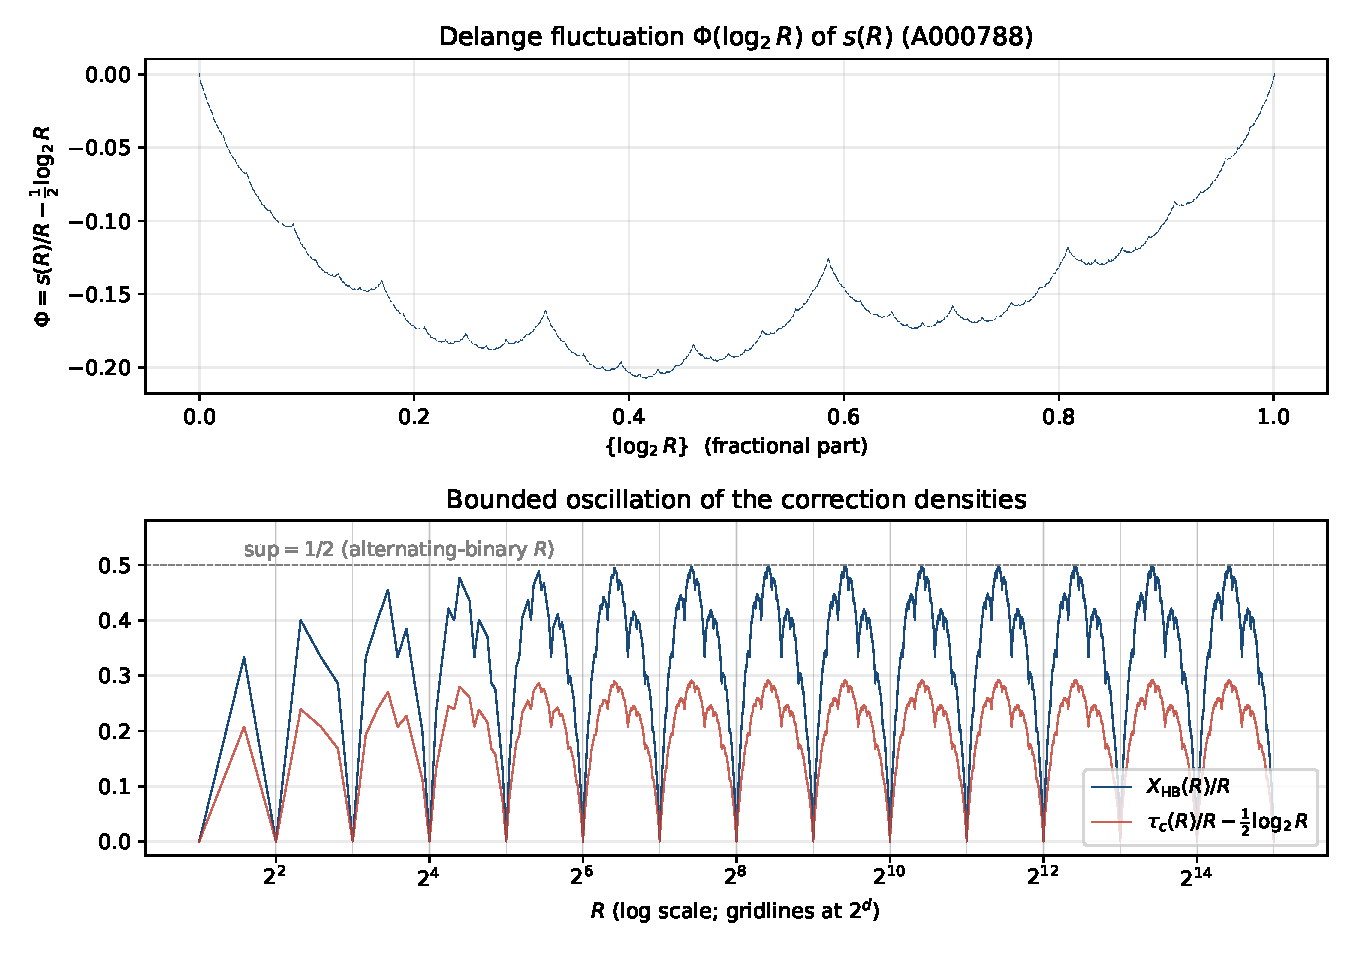
\includegraphics[width=0.92\textwidth]{../assets/out/delange-structure.pdf}
	\caption{Top: the Delange fluctuation $\Phi(\log_2 R)$
		of~\eqref{eq:delange}, computed from $\Eseq(R)$ for
		$256 \le R \le 2^{20}$ and plotted against $\{\log_2 R\}$; the
		self-similar, nowhere-differentiable profile is characteristic of
		radix-$2$ digital sums. Bottom: the centered correction density
		$\Cconst(R)/R - \tfrac{1}{2}\log_2 R$ and the cross-collision density
		$X(\mathrm{HB}_R)/R$ of Corollary~\ref{cor:densities} for
		$2 \le R \le 2^{15}$; both are bounded oscillations in $\log_2 R$,
		vanishing at every power of two (gridlines). The dashed line marks the
		empirical supremum $1/2$ of the cross-collision density, approached
		along the alternating-binary integers
		$R = \lceil 2^{d+1}/3 \rceil$ (e.g.\ $R = 43691 =
			(1010101010101011)_2$ attains $X/R > 0.49998$).}
	\label{fig:delange}
\end{figure}

\begin{remark}[Extremal densities]\label{rem:extremal}
	Numerically, $\sup_R X(\mathrm{HB}_R)/R = \tfrac{1}{2}$ for all sampled
	$R < 2^{16}$ (Figure~\ref{fig:delange}), approached along the
	alternating-binary integers $R = \lceil 2^{d+1}/3\rceil$, which are the
	classical extremizers of the Delange fluctuation; we record this as
	numerical evidence rather than a proven exact supremum, since we have
	not derived it from the Trollope--Delange expansion. The
	graph-theoretic reading is pleasing: the Hamming ball's shielding
	$4$-cycles appear, in this numerical range, to never exceed one per two
	vertices; the largest observed densities occur along the
	alternating-binary integers described above, and they disappear entirely when the ball
	closes into a full subcube.
\end{remark}

\begin{remark}[Relation to the Asymptotic Penalty]\label{rem:penalty-analogy}
	Corollary~\ref{cor:densities} quantifies exactly the $O_R(1)$ terms of
	Theorem~\ref{them:penalty}: in the boundary
	formula~\eqref{eq:extraconnectivity}, the dimension scaling contributes
	the exact linear term in $(n-k)$, while the correction density
	$\Cconst(R)/R$ splits, per~\eqref{eq:C-density}, into a logarithmic trend
	$\tfrac{1}{2}\log_2 R$ plus the bounded oscillation $\Psi(u) -
	\Phi(\log_2 R)$ that carries its entire remaining $R$-dependence.
	Readers
	familiar with analytic
	combinatorics~\cite{wilf2006generatingfunctionology} may recognize the
	division of labor: as in singularity analysis, where a dominant pole
	dictates growth and the remaining analytic part contributes bounded
	corrections, the identity of Theorem~\ref{them:penalty} separates the
	dominant $\Delta D \cdot (n-k)$ term from a topology-dependent constant
	--- though here the separation is an exact finite identity, proved
	directly in the discrete domain, rather than an asymptotic extraction.
\end{remark}
  immediately BEFORE  \section{The Fracture Gap
% and Defect Continuity}  (currently line ~702), so it follows the Asymptotic
% Penalty section whose coefficients it analyzes.
% Requires: figure at ../assets/out/delange-structure.pdf
%           (regenerate: scripts/gen_delange_figure.py)
% New bib entries: see references-additions.bib (trollope1968explicit,
% delange1975somme, allouche1992ring, allouche2003automatic,
% adamczewski2017problem, wilf2006generatingfunctionology).
% The generating-function/Mahler identities (Props ogf, mahler) and the
% closed-form/density decomposition are checked by
% scripts/verify_gf_identities.py for finitely many R (series to order 600;
% density decomposition for R < 2^16; closed forms over their scripted ranges).
% consistency check, not a proof: it does not (and cannot) establish the
% section's genuinely analytic claims — nowhere-differentiability in
% Theorem them:delange and transcendence in Corollary cor:transcend rest on
% their own arguments/citations; the supremum in Remark rem:extremal is not
% proven at all, and is presented there only as numerical evidence.
% ============================================================================

\section{Analytic Structure of the Boundary Coefficients}\label{sec:analytic}

The extraconnectivity formula~\eqref{eq:extraconnectivity} is governed by two
integer sequences: the cumulative binary weight $\Eseq(R)$ (OEIS A000788) and
the correction constant $\Cconst(R)$, linked by the closed
form~\eqref{eq:cconst}. In this section we place these coefficients in their
classical analytic context: we derive their ordinary generating functions in
the style of Wilf~\cite{wilf2006generatingfunctionology}, exhibit an exact
Mahler functional equation certifying that no linear-recurrence
(rational-generating-function) closed form for them can exist, and import the
Trollope--Delange theorem to give the exact asymptotics of the boundary
formula, including a continuous, nowhere-differentiable periodic fluctuation
that the correction density inherits. Everything in this section is an
unconditional statement about the integer sequences themselves; it does not
depend on Propositions~\ref{prop:universal} or~\ref{prop:hb-eval}. Via
Proposition~\ref{prop:hb-eval}, the difference $\Cconst(R) - \Eseq(R)$ acquires
its graph-theoretic reading as the cross-collision count $X(\mathrm{HB}_R)$,
and we use that notation for it below.

\subsection{Ordinary generating functions}

Write $s_2(i) = \mathrm{popcount}(i)$ for the binary digit sum, so
$\Eseq(R) = \sum_{i<R} s_2(i)$, and abbreviate the ceiling-log summand of
Definition~\ref{def:constants} by
$\lambda(i) = \lceil \log_2(i+1) \rceil$ (the bit length of $i$).

\begin{proposition}[Generating functions of the coefficients]\label{prop:ogf}
	As formal power series,
	\begin{align}
		\sum_{i \ge 0} s_2(i)\, x^i
		 & = \frac{1}{1-x} \sum_{j \ge 0} \frac{x^{2^j}}{1+x^{2^j}},
		\label{eq:ogf-s2}                                             \\
		\sum_{R \ge 0} \Eseq(R)\, x^R
		 & = \frac{x}{(1-x)^2} \sum_{j \ge 0} \frac{x^{2^j}}{1+x^{2^j}},
		\label{eq:ogf-E}                                              \\
		\sum_{R \ge 0} \Cconst(R)\, x^R
		 & = \frac{x^2}{(1-x)^2}
		+ \frac{x}{(1-x)^2} \sum_{j \ge 0} \frac{x^{2^{j+1}}}{1+x^{2^j}}.
		\label{eq:ogf-C}
	\end{align}
\end{proposition}

\begin{proof}
	The indicator of ``bit $j$ of $i$ is set'' is periodic in $i$ with period
	$2^{j+1}$ and pattern $0^{2^j} 1^{2^j}$; summing the geometric series over
	one period and over all periods gives
	$\sum_i [\,\text{bit } j \text{ of } i\,]\, x^i
		= x^{2^j} \frac{1-x^{2^j}}{1-x} \cdot \frac{1}{1-x^{2^{j+1}}}
		= \frac{x^{2^j}}{(1-x)(1+x^{2^j})}$.
	Summing over $j$ yields~\eqref{eq:ogf-s2} since
	$s_2 = \sum_j [\,\text{bit } j\,]$. Partial summation is multiplication by
	$x/(1-x)$: if $A(x) = \sum_i a_i x^i$ then
	$\sum_R \big(\sum_{i<R} a_i\big) x^R = \frac{x}{1-x} A(x)$, giving~\eqref{eq:ogf-E}.
	For~\eqref{eq:ogf-C}, the same period argument applied to the indicator
	$[\lambda(i) > j] = [i \ge 2^j]$ gives
	$\sum_i \lambda(i) x^i = \frac{1}{1-x}\sum_{j\ge0} x^{2^j}$, hence
	$\sum_R \big(\sum_{i<R}\lambda(i)\big) x^R = \frac{x}{(1-x)^2}\sum_j x^{2^j}$;
	combining with $\sum_{R \ge 1} (R-1)x^R = \frac{x^2}{(1-x)^2}$
	and~\eqref{eq:ogf-E} per Definition~\ref{def:constants}, the
	$\Eseq$-series cancels term-by-term against the $\lambda$-series via
	$\frac{x^{2^j}}{1} - \frac{x^{2^j}}{1+x^{2^j}} = \frac{x^{2^{j+1}}}{1+x^{2^j}}$.
\end{proof}

\subsection{A Mahler functional equation, and why no simpler closed form exists}

The radix-2 recurrences $\Eseq(2m) = 2\Eseq(m) + m$ and
$\Eseq(2m+1) = \Eseq(m) + \Eseq(m+1) + m$ that drive
Lemma~\ref{lem:subadditivity} translate, in the generating-function domain,
into a functional equation of Mahler type~--- the classical algebraic home of
divide-and-conquer sequences.

\begin{proposition}[Mahler equation]\label{prop:mahler}
	Let $S(x) = \sum_{i\ge0} s_2(i)x^i$ and $F(x) = \sum_R \Eseq(R) x^R$. Then
	\begin{equation}\label{eq:mahler}
		S(x) = (1+x)\, S(x^2) + \frac{x}{1-x^2},
		\qquad\text{equivalently}\qquad
		x\,F(x) = (1+x)^2\, F(x^2) + \frac{x^3}{(1-x)(1-x^2)} .
	\end{equation}
	In particular $S$ and $F$ are $2$-Mahler functions of order one, and
	$s_2$, $\Eseq$, and (via~\eqref{eq:cconst}) $\Cconst$ are $2$-regular
	sequences in the sense of
	Allouche--Shallit~\cite{allouche1992ring,allouche2003automatic}.
\end{proposition}

\begin{proof}
	Splitting $S$ over even and odd indices and applying
	$s_2(2m) = s_2(m)$, $s_2(2m+1) = s_2(m) + 1$ gives
	$S(x) = S(x^2) + x\,S(x^2) + x\sum_{m\ge0} x^{2m}$, which
	is~\eqref{eq:mahler}; the $F$-form follows from
	$F(x) = \frac{x}{1-x} S(x)$. Regularity of $s_2$ is the textbook example
	in~\cite{allouche1992ring}; the ring of $2$-regular sequences is closed
	under running sums (giving $\Eseq$). For $\Cconst$, write
	$d = \lceil \log_2 R \rceil$, the bit length of $R-1$ (for $R \ge 1$); it is a
	standard $2$-regular sequence~\cite{allouche1992ring}, as is
	$2^{d} = 2^{\lceil \log_2 R \rceil}$ (the round-up-to-a-power-of-$2$
	sequence), and $R$ is $2$-regular as a polynomial sequence; since the
	$2$-regular sequences form a ring (closed under both sums and products),
	$R(d{+}1) - 2^d$ is $2$-regular, and hence so is
	$\Cconst = R(d{+}1) - 2^d - \Eseq$ by~\eqref{eq:cconst}.
\end{proof}

The $2$-regular matrix representation is exactly what the characterization
engine exploits: \texttt{predict.cpp} evaluates $\Eseq(R)$ in $O(\log R)$ by
recursing on the binary expansion (Appendix~\ref{app:engine}), which is the
operational form of Proposition~\ref{prop:mahler}.

\begin{corollary}[No linear-recurrence closed form]\label{cor:transcend}
	$F(x)$ is transcendental over $\mathbb{Q}(x)$. Consequently $\Eseq(R)$
	(and hence $\Cconst(R)$) satisfies no linear recurrence with constant
	coefficients: the correction constants of
	Theorem~\ref{them:main} are not expressible by any rational generating
	function or polynomial-exponential closed form.
\end{corollary}

\begin{proof}
	We first show: no sequence of the form $a(R) = \tfrac{1}{2}R\log_2 R +
	O(R)$ is $C$-finite. Suppose $a(R) = \sum_i p_i(R)\lambda_i^R$ for
	finitely many algebraic $\lambda_i$ and polynomials $p_i$, not all zero.
	By Cauchy--Hadamard applied to the ordinary generating function of $a$,
	its radius of convergence is $1/\rho$ with $\rho = \max_i |\lambda_i|$,
	and $a(R)^{1/R} \to 1$ since $a(R) = \Theta(R\log R)$; hence $\rho = 1$,
	so every $|\lambda_i| \le 1$. Let $K \ge 0$ be the largest degree of
	$p_i$ among indices with $|\lambda_i| = 1$ (such indices exist, else
	$a(R) \to 0$), and let $h(R) = \sum_{|\lambda_i|=1} \mathrm{lead}(p_i)
	\lambda_i^R$ collect the corresponding leading coefficients; every other
	term is $o(R^K)$, so $a(R)/R^K - h(R) \to 0$. As $h$ is a nonzero finite
	sum of unit-modulus exponentials, orthogonality of distinct characters
	gives $\frac{1}{N}\sum_{R<N} |h(R)|^2 \to \sum_{|\lambda_i|=1}
	|\mathrm{lead}(p_i)|^2 > 0$, so $h$ is bounded (a finite trigonometric
	sum) but does not tend to $0$ in mean square; in particular $a(R)/R^K$
	is bounded and $\limsup_R |a(R)|/R^K > 0$. But $a(R)/R^K =
	\tfrac{1}{2}R^{1-K}\log_2 R + O(R^{1-K})$ tends to $\infty$ for $K \le 1$
	(contradicting boundedness) and to $0$ for $K \ge 2$ (contradicting
	positive limsup). No $K$ survives, so $a$ is not $C$-finite.

	Since $\Eseq(R) = \tfrac{1}{2}R\log_2 R + O(R)$ (Theorem~\ref{them:delange}
	below), $\Eseq$ is not $C$-finite by the above, so $F$ is not rational
	(a rational $F$ would make $\Eseq$ eventually satisfy a linear recurrence
	with constant coefficients, i.e.\ be $C$-finite). The identical growth
	class applies to $\Cconst$: writing $d = \lceil \log_2 R \rceil$,
	\eqref{eq:cconst} gives $\Cconst(R) = R(d{+}1) - 2^d - \Eseq(R)$, and
	since $2^{d-1} < R \le 2^d$ we have $2^d = \Theta(R)$, so
	$R(d{+}1) - 2^d = R\log_2 R + O(R)$; combined with the expansion of
	$\Eseq$ this gives $\Cconst(R) = \tfrac{1}{2}R\log_2 R + O(R)$, so
	$\Cconst$ is not $C$-finite either. A Mahler function that is algebraic
	over $\mathbb{Q}(x)$ is rational by the theorem of Adamczewski and
	Bell~\cite{adamczewski2017problem}; since $F$ satisfies~\eqref{eq:mahler}
	and is irrational, it is transcendental.
\end{proof}

\subsection{Exact asymptotics: the Trollope--Delange fluctuation}

\begin{theorem}[Trollope~\cite{trollope1968explicit};
		Delange~\cite{delange1975somme}]\label{them:delange}
	There is a continuous, nowhere-differentiable function
	$\Phi \colon \mathbb{R} \to \mathbb{R}$ of period $1$ such that for all
	$R \ge 1$,
	\begin{equation}\label{eq:delange}
		\Eseq(R) = \tfrac{1}{2} R \log_2 R + R\,\Phi(\log_2 R).
	\end{equation}
	The Fourier coefficients of $\Phi$ are known explicitly and involve the
	values of the Riemann zeta function at the points
	$2\pi i k/\log 2$ on the imaginary axis~\cite{delange1975somme}.
\end{theorem}

\begin{corollary}[Fluctuation of the correction densities]\label{cor:densities}
	Let $u = \{\log_2 R\}$ denote the fractional part and set
	$\Psi(u) = 2 - u - 2^{1-u}$. Then for all $R \ge 2$,
	\begin{align}
		\frac{\Cconst(R)}{R}
		 & = \tfrac{1}{2}\log_2 R \;+\; \Psi(u) \;-\; \Phi(\log_2 R),
		\label{eq:C-density}                                        \\
		\frac{X(\mathrm{HB}_R)}{R} \;=\; \frac{\Cconst(R)-\Eseq(R)}{R}
		 & = \Psi(u) \;-\; 2\,\Phi(\log_2 R).
		\label{eq:X-density}
	\end{align}
	In particular the cross-collision density
	$(\Cconst(R)-\Eseq(R))/R$ is a \emph{bounded}, purely oscillatory function
	of $\log_2 R$: it carries no growing term, vanishes exactly at the powers
	of two ($\Psi(0) = \Phi(d) = 0$), and is strictly positive elsewhere.
\end{corollary}

\begin{proof}
	Write $d = \lceil \log_2 R \rceil$, so for $R$ not a power of two
	$d = \log_2 R - u + 1$, and directly from the closed
	form~\eqref{eq:cconst},
	$\Cconst(R)/R = (d+1) - 2^d/R - \Eseq(R)/R
		= \log_2 R + (2 - u - 2^{1-u}) - \Eseq(R)/R$;
	substituting~\eqref{eq:delange} gives~\eqref{eq:C-density}, and
	subtracting $\Eseq(R)/R$ once more gives~\eqref{eq:X-density}. At
	$R = 2^d$ both sides agree in the limit $u \to 0^+$ and equal
	$\Cconst(2^d)/2^d - \tfrac{d}{2} = 0$, recovering
	$\Cconst(2^d) = \Eseq(2^d)$ and $X(\mathrm{HB}_{2^d}) = 0$. Boundedness
	of~\eqref{eq:X-density} follows since $\Psi$ and $\Phi$ are continuous and
	periodic; positivity away from powers of two is
	Proposition~\ref{prop:hb-eval}'s
	$X(\mathrm{HB}_R) = \Cconst(R) - \Eseq(R) \ge 0$ together with the strict
	inequality visible in the closed form.
\end{proof}

\begin{figure}[ht]
	\centering
	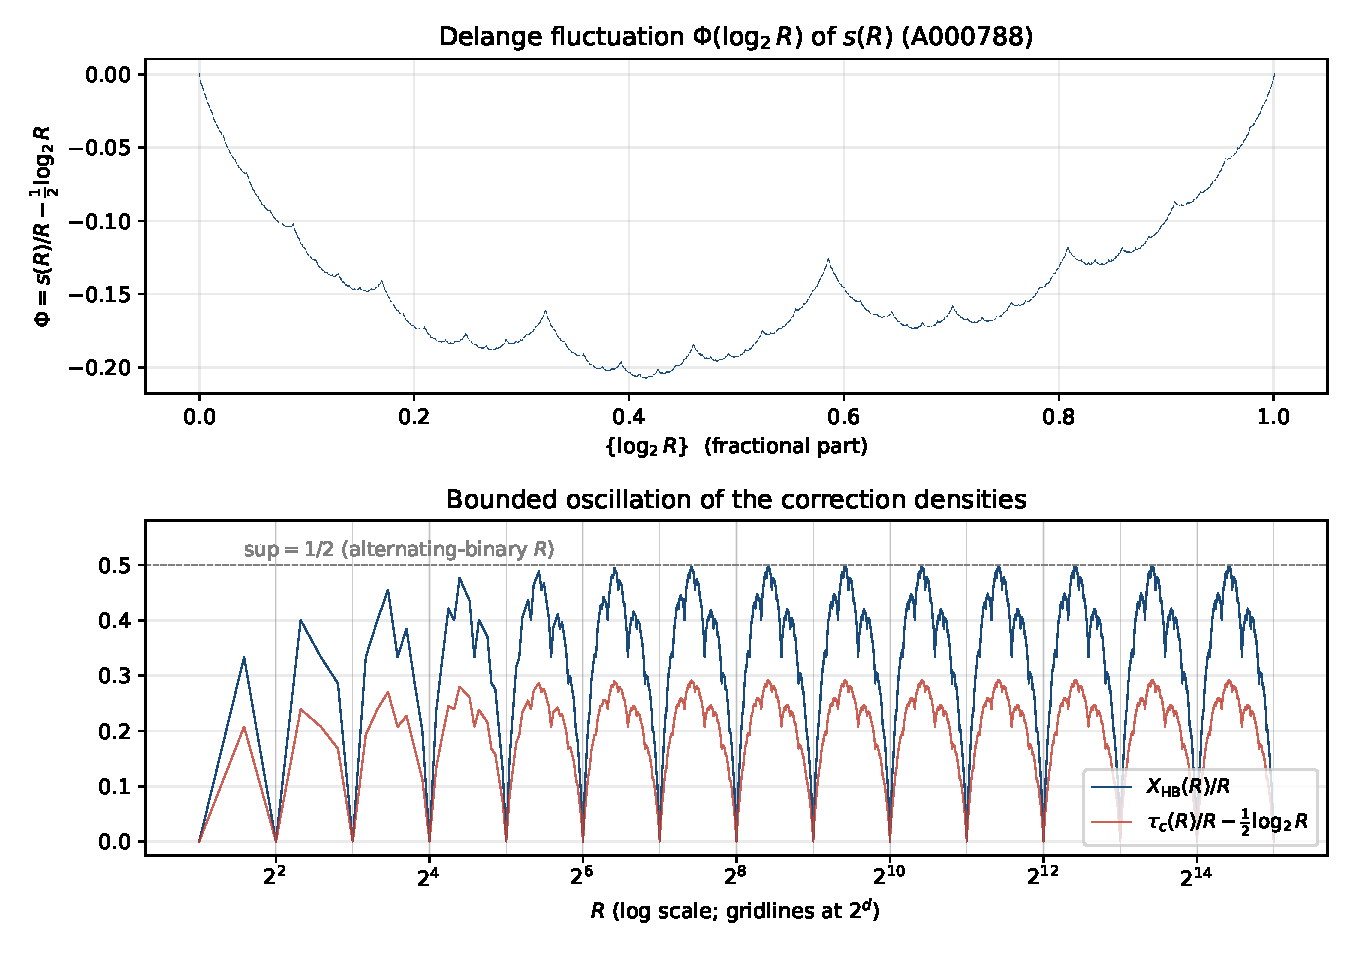
\includegraphics[width=0.92\textwidth]{../assets/out/delange-structure.pdf}
	\caption{Top: the Delange fluctuation $\Phi(\log_2 R)$
		of~\eqref{eq:delange}, computed from $\Eseq(R)$ for
		$256 \le R \le 2^{20}$ and plotted against $\{\log_2 R\}$; the
		self-similar, nowhere-differentiable profile is characteristic of
		radix-$2$ digital sums. Bottom: the centered correction density
		$\Cconst(R)/R - \tfrac{1}{2}\log_2 R$ and the cross-collision density
		$X(\mathrm{HB}_R)/R$ of Corollary~\ref{cor:densities} for
		$2 \le R \le 2^{15}$; both are bounded oscillations in $\log_2 R$,
		vanishing at every power of two (gridlines). The dashed line marks the
		empirical supremum $1/2$ of the cross-collision density, approached
		along the alternating-binary integers
		$R = \lceil 2^{d+1}/3 \rceil$ (e.g.\ $R = 43691 =
			(1010101010101011)_2$ attains $X/R > 0.49998$).}
	\label{fig:delange}
\end{figure}

\begin{remark}[Extremal densities]\label{rem:extremal}
	Numerically, $\sup_R X(\mathrm{HB}_R)/R = \tfrac{1}{2}$ for all sampled
	$R < 2^{16}$ (Figure~\ref{fig:delange}), approached along the
	alternating-binary integers $R = \lceil 2^{d+1}/3\rceil$, which are the
	classical extremizers of the Delange fluctuation; we record this as
	numerical evidence rather than a proven exact supremum, since we have
	not derived it from the Trollope--Delange expansion. The
	graph-theoretic reading is pleasing: the Hamming ball's shielding
	$4$-cycles appear, in this numerical range, to never exceed one per two
	vertices; the largest observed densities occur along the
	alternating-binary integers described above, and they disappear entirely when the ball
	closes into a full subcube.
\end{remark}

\begin{remark}[Relation to the Asymptotic Penalty]\label{rem:penalty-analogy}
	Corollary~\ref{cor:densities} quantifies exactly the $O_R(1)$ terms of
	Theorem~\ref{them:penalty}: in the boundary
	formula~\eqref{eq:extraconnectivity}, the dimension scaling contributes
	the exact linear term in $(n-k)$, while the correction density
	$\Cconst(R)/R$ splits, per~\eqref{eq:C-density}, into a logarithmic trend
	$\tfrac{1}{2}\log_2 R$ plus the bounded oscillation $\Psi(u) -
	\Phi(\log_2 R)$ that carries its entire remaining $R$-dependence.
	Readers
	familiar with analytic
	combinatorics~\cite{wilf2006generatingfunctionology} may recognize the
	division of labor: as in singularity analysis, where a dominant pole
	dictates growth and the remaining analytic part contributes bounded
	corrections, the identity of Theorem~\ref{them:penalty} separates the
	dominant $\Delta D \cdot (n-k)$ term from a topology-dependent constant
	--- though here the separation is an exact finite identity, proved
	directly in the discrete domain, rather than an asymptotic extraction.
\end{remark}
  immediately BEFORE  \section{The Fracture Gap
% and Defect Continuity}  (currently line ~702), so it follows the Asymptotic
% Penalty section whose coefficients it analyzes.
% Requires: figure at ../assets/out/delange-structure.pdf
%           (regenerate: scripts/gen_delange_figure.py)
% New bib entries: see references-additions.bib (trollope1968explicit,
% delange1975somme, allouche1992ring, allouche2003automatic,
% adamczewski2017problem, wilf2006generatingfunctionology).
% The generating-function/Mahler identities (Props ogf, mahler) and the
% closed-form/density decomposition are checked by
% scripts/verify_gf_identities.py for finitely many R (series to order 600;
% density decomposition for R < 2^16; closed forms over their scripted ranges).
% consistency check, not a proof: it does not (and cannot) establish the
% section's genuinely analytic claims — nowhere-differentiability in
% Theorem them:delange and transcendence in Corollary cor:transcend rest on
% their own arguments/citations; the supremum in Remark rem:extremal is not
% proven at all, and is presented there only as numerical evidence.
% ============================================================================

\section{Analytic Structure of the Boundary Coefficients}\label{sec:analytic}

The extraconnectivity formula~\eqref{eq:extraconnectivity} is governed by two
integer sequences: the cumulative binary weight $\Eseq(R)$ (OEIS A000788) and
the correction constant $\Cconst(R)$, linked by the closed
form~\eqref{eq:cconst}. In this section we place these coefficients in their
classical analytic context: we derive their ordinary generating functions in
the style of Wilf~\cite{wilf2006generatingfunctionology}, exhibit an exact
Mahler functional equation certifying that no linear-recurrence
(rational-generating-function) closed form for them can exist, and import the
Trollope--Delange theorem to give the exact asymptotics of the boundary
formula, including a continuous, nowhere-differentiable periodic fluctuation
that the correction density inherits. Everything in this section is an
unconditional statement about the integer sequences themselves; it does not
depend on Propositions~\ref{prop:universal} or~\ref{prop:hb-eval}. Via
Proposition~\ref{prop:hb-eval}, the difference $\Cconst(R) - \Eseq(R)$ acquires
its graph-theoretic reading as the cross-collision count $X(\mathrm{HB}_R)$,
and we use that notation for it below.

\subsection{Ordinary generating functions}

Write $s_2(i) = \mathrm{popcount}(i)$ for the binary digit sum, so
$\Eseq(R) = \sum_{i<R} s_2(i)$, and abbreviate the ceiling-log summand of
Definition~\ref{def:constants} by
$\lambda(i) = \lceil \log_2(i+1) \rceil$ (the bit length of $i$).

\begin{proposition}[Generating functions of the coefficients]\label{prop:ogf}
	As formal power series,
	\begin{align}
		\sum_{i \ge 0} s_2(i)\, x^i
		 & = \frac{1}{1-x} \sum_{j \ge 0} \frac{x^{2^j}}{1+x^{2^j}},
		\label{eq:ogf-s2}                                             \\
		\sum_{R \ge 0} \Eseq(R)\, x^R
		 & = \frac{x}{(1-x)^2} \sum_{j \ge 0} \frac{x^{2^j}}{1+x^{2^j}},
		\label{eq:ogf-E}                                              \\
		\sum_{R \ge 0} \Cconst(R)\, x^R
		 & = \frac{x^2}{(1-x)^2}
		+ \frac{x}{(1-x)^2} \sum_{j \ge 0} \frac{x^{2^{j+1}}}{1+x^{2^j}}.
		\label{eq:ogf-C}
	\end{align}
\end{proposition}

\begin{proof}
	The indicator of ``bit $j$ of $i$ is set'' is periodic in $i$ with period
	$2^{j+1}$ and pattern $0^{2^j} 1^{2^j}$; summing the geometric series over
	one period and over all periods gives
	$\sum_i [\,\text{bit } j \text{ of } i\,]\, x^i
		= x^{2^j} \frac{1-x^{2^j}}{1-x} \cdot \frac{1}{1-x^{2^{j+1}}}
		= \frac{x^{2^j}}{(1-x)(1+x^{2^j})}$.
	Summing over $j$ yields~\eqref{eq:ogf-s2} since
	$s_2 = \sum_j [\,\text{bit } j\,]$. Partial summation is multiplication by
	$x/(1-x)$: if $A(x) = \sum_i a_i x^i$ then
	$\sum_R \big(\sum_{i<R} a_i\big) x^R = \frac{x}{1-x} A(x)$, giving~\eqref{eq:ogf-E}.
	For~\eqref{eq:ogf-C}, the same period argument applied to the indicator
	$[\lambda(i) > j] = [i \ge 2^j]$ gives
	$\sum_i \lambda(i) x^i = \frac{1}{1-x}\sum_{j\ge0} x^{2^j}$, hence
	$\sum_R \big(\sum_{i<R}\lambda(i)\big) x^R = \frac{x}{(1-x)^2}\sum_j x^{2^j}$;
	combining with $\sum_{R \ge 1} (R-1)x^R = \frac{x^2}{(1-x)^2}$
	and~\eqref{eq:ogf-E} per Definition~\ref{def:constants}, the
	$\Eseq$-series cancels term-by-term against the $\lambda$-series via
	$\frac{x^{2^j}}{1} - \frac{x^{2^j}}{1+x^{2^j}} = \frac{x^{2^{j+1}}}{1+x^{2^j}}$.
\end{proof}

\subsection{A Mahler functional equation, and why no simpler closed form exists}

The radix-2 recurrences $\Eseq(2m) = 2\Eseq(m) + m$ and
$\Eseq(2m+1) = \Eseq(m) + \Eseq(m+1) + m$ that drive
Lemma~\ref{lem:subadditivity} translate, in the generating-function domain,
into a functional equation of Mahler type~--- the classical algebraic home of
divide-and-conquer sequences.

\begin{proposition}[Mahler equation]\label{prop:mahler}
	Let $S(x) = \sum_{i\ge0} s_2(i)x^i$ and $F(x) = \sum_R \Eseq(R) x^R$. Then
	\begin{equation}\label{eq:mahler}
		S(x) = (1+x)\, S(x^2) + \frac{x}{1-x^2},
		\qquad\text{equivalently}\qquad
		x\,F(x) = (1+x)^2\, F(x^2) + \frac{x^3}{(1-x)(1-x^2)} .
	\end{equation}
	In particular $S$ and $F$ are $2$-Mahler functions of order one, and
	$s_2$, $\Eseq$, and (via~\eqref{eq:cconst}) $\Cconst$ are $2$-regular
	sequences in the sense of
	Allouche--Shallit~\cite{allouche1992ring,allouche2003automatic}.
\end{proposition}

\begin{proof}
	Splitting $S$ over even and odd indices and applying
	$s_2(2m) = s_2(m)$, $s_2(2m+1) = s_2(m) + 1$ gives
	$S(x) = S(x^2) + x\,S(x^2) + x\sum_{m\ge0} x^{2m}$, which
	is~\eqref{eq:mahler}; the $F$-form follows from
	$F(x) = \frac{x}{1-x} S(x)$. Regularity of $s_2$ is the textbook example
	in~\cite{allouche1992ring}; the ring of $2$-regular sequences is closed
	under running sums (giving $\Eseq$). For $\Cconst$, write
	$d = \lceil \log_2 R \rceil$, the bit length of $R-1$ (for $R \ge 1$); it is a
	standard $2$-regular sequence~\cite{allouche1992ring}, as is
	$2^{d} = 2^{\lceil \log_2 R \rceil}$ (the round-up-to-a-power-of-$2$
	sequence), and $R$ is $2$-regular as a polynomial sequence; since the
	$2$-regular sequences form a ring (closed under both sums and products),
	$R(d{+}1) - 2^d$ is $2$-regular, and hence so is
	$\Cconst = R(d{+}1) - 2^d - \Eseq$ by~\eqref{eq:cconst}.
\end{proof}

The $2$-regular matrix representation is exactly what the characterization
engine exploits: \texttt{predict.cpp} evaluates $\Eseq(R)$ in $O(\log R)$ by
recursing on the binary expansion (Appendix~\ref{app:engine}), which is the
operational form of Proposition~\ref{prop:mahler}.

\begin{corollary}[No linear-recurrence closed form]\label{cor:transcend}
	$F(x)$ is transcendental over $\mathbb{Q}(x)$. Consequently $\Eseq(R)$
	(and hence $\Cconst(R)$) satisfies no linear recurrence with constant
	coefficients: the correction constants of
	Theorem~\ref{them:main} are not expressible by any rational generating
	function or polynomial-exponential closed form.
\end{corollary}

\begin{proof}
	We first show: no sequence of the form $a(R) = \tfrac{1}{2}R\log_2 R +
	O(R)$ is $C$-finite. Suppose $a(R) = \sum_i p_i(R)\lambda_i^R$ for
	finitely many algebraic $\lambda_i$ and polynomials $p_i$, not all zero.
	By Cauchy--Hadamard applied to the ordinary generating function of $a$,
	its radius of convergence is $1/\rho$ with $\rho = \max_i |\lambda_i|$,
	and $a(R)^{1/R} \to 1$ since $a(R) = \Theta(R\log R)$; hence $\rho = 1$,
	so every $|\lambda_i| \le 1$. Let $K \ge 0$ be the largest degree of
	$p_i$ among indices with $|\lambda_i| = 1$ (such indices exist, else
	$a(R) \to 0$), and let $h(R) = \sum_{|\lambda_i|=1} \mathrm{lead}(p_i)
	\lambda_i^R$ collect the corresponding leading coefficients; every other
	term is $o(R^K)$, so $a(R)/R^K - h(R) \to 0$. As $h$ is a nonzero finite
	sum of unit-modulus exponentials, orthogonality of distinct characters
	gives $\frac{1}{N}\sum_{R<N} |h(R)|^2 \to \sum_{|\lambda_i|=1}
	|\mathrm{lead}(p_i)|^2 > 0$, so $h$ is bounded (a finite trigonometric
	sum) but does not tend to $0$ in mean square; in particular $a(R)/R^K$
	is bounded and $\limsup_R |a(R)|/R^K > 0$. But $a(R)/R^K =
	\tfrac{1}{2}R^{1-K}\log_2 R + O(R^{1-K})$ tends to $\infty$ for $K \le 1$
	(contradicting boundedness) and to $0$ for $K \ge 2$ (contradicting
	positive limsup). No $K$ survives, so $a$ is not $C$-finite.

	Since $\Eseq(R) = \tfrac{1}{2}R\log_2 R + O(R)$ (Theorem~\ref{them:delange}
	below), $\Eseq$ is not $C$-finite by the above, so $F$ is not rational
	(a rational $F$ would make $\Eseq$ eventually satisfy a linear recurrence
	with constant coefficients, i.e.\ be $C$-finite). The identical growth
	class applies to $\Cconst$: writing $d = \lceil \log_2 R \rceil$,
	\eqref{eq:cconst} gives $\Cconst(R) = R(d{+}1) - 2^d - \Eseq(R)$, and
	since $2^{d-1} < R \le 2^d$ we have $2^d = \Theta(R)$, so
	$R(d{+}1) - 2^d = R\log_2 R + O(R)$; combined with the expansion of
	$\Eseq$ this gives $\Cconst(R) = \tfrac{1}{2}R\log_2 R + O(R)$, so
	$\Cconst$ is not $C$-finite either. A Mahler function that is algebraic
	over $\mathbb{Q}(x)$ is rational by the theorem of Adamczewski and
	Bell~\cite{adamczewski2017problem}; since $F$ satisfies~\eqref{eq:mahler}
	and is irrational, it is transcendental.
\end{proof}

\subsection{Exact asymptotics: the Trollope--Delange fluctuation}

\begin{theorem}[Trollope~\cite{trollope1968explicit};
		Delange~\cite{delange1975somme}]\label{them:delange}
	There is a continuous, nowhere-differentiable function
	$\Phi \colon \mathbb{R} \to \mathbb{R}$ of period $1$ such that for all
	$R \ge 1$,
	\begin{equation}\label{eq:delange}
		\Eseq(R) = \tfrac{1}{2} R \log_2 R + R\,\Phi(\log_2 R).
	\end{equation}
	The Fourier coefficients of $\Phi$ are known explicitly and involve the
	values of the Riemann zeta function at the points
	$2\pi i k/\log 2$ on the imaginary axis~\cite{delange1975somme}.
\end{theorem}

\begin{corollary}[Fluctuation of the correction densities]\label{cor:densities}
	Let $u = \{\log_2 R\}$ denote the fractional part and set
	$\Psi(u) = 2 - u - 2^{1-u}$. Then for all $R \ge 2$,
	\begin{align}
		\frac{\Cconst(R)}{R}
		 & = \tfrac{1}{2}\log_2 R \;+\; \Psi(u) \;-\; \Phi(\log_2 R),
		\label{eq:C-density}                                        \\
		\frac{X(\mathrm{HB}_R)}{R} \;=\; \frac{\Cconst(R)-\Eseq(R)}{R}
		 & = \Psi(u) \;-\; 2\,\Phi(\log_2 R).
		\label{eq:X-density}
	\end{align}
	In particular the cross-collision density
	$(\Cconst(R)-\Eseq(R))/R$ is a \emph{bounded}, purely oscillatory function
	of $\log_2 R$: it carries no growing term, vanishes exactly at the powers
	of two ($\Psi(0) = \Phi(d) = 0$), and is strictly positive elsewhere.
\end{corollary}

\begin{proof}
	Write $d = \lceil \log_2 R \rceil$, so for $R$ not a power of two
	$d = \log_2 R - u + 1$, and directly from the closed
	form~\eqref{eq:cconst},
	$\Cconst(R)/R = (d+1) - 2^d/R - \Eseq(R)/R
		= \log_2 R + (2 - u - 2^{1-u}) - \Eseq(R)/R$;
	substituting~\eqref{eq:delange} gives~\eqref{eq:C-density}, and
	subtracting $\Eseq(R)/R$ once more gives~\eqref{eq:X-density}. At
	$R = 2^d$ both sides agree in the limit $u \to 0^+$ and equal
	$\Cconst(2^d)/2^d - \tfrac{d}{2} = 0$, recovering
	$\Cconst(2^d) = \Eseq(2^d)$ and $X(\mathrm{HB}_{2^d}) = 0$. Boundedness
	of~\eqref{eq:X-density} follows since $\Psi$ and $\Phi$ are continuous and
	periodic; positivity away from powers of two is
	Proposition~\ref{prop:hb-eval}'s
	$X(\mathrm{HB}_R) = \Cconst(R) - \Eseq(R) \ge 0$ together with the strict
	inequality visible in the closed form.
\end{proof}

\begin{figure}[ht]
	\centering
	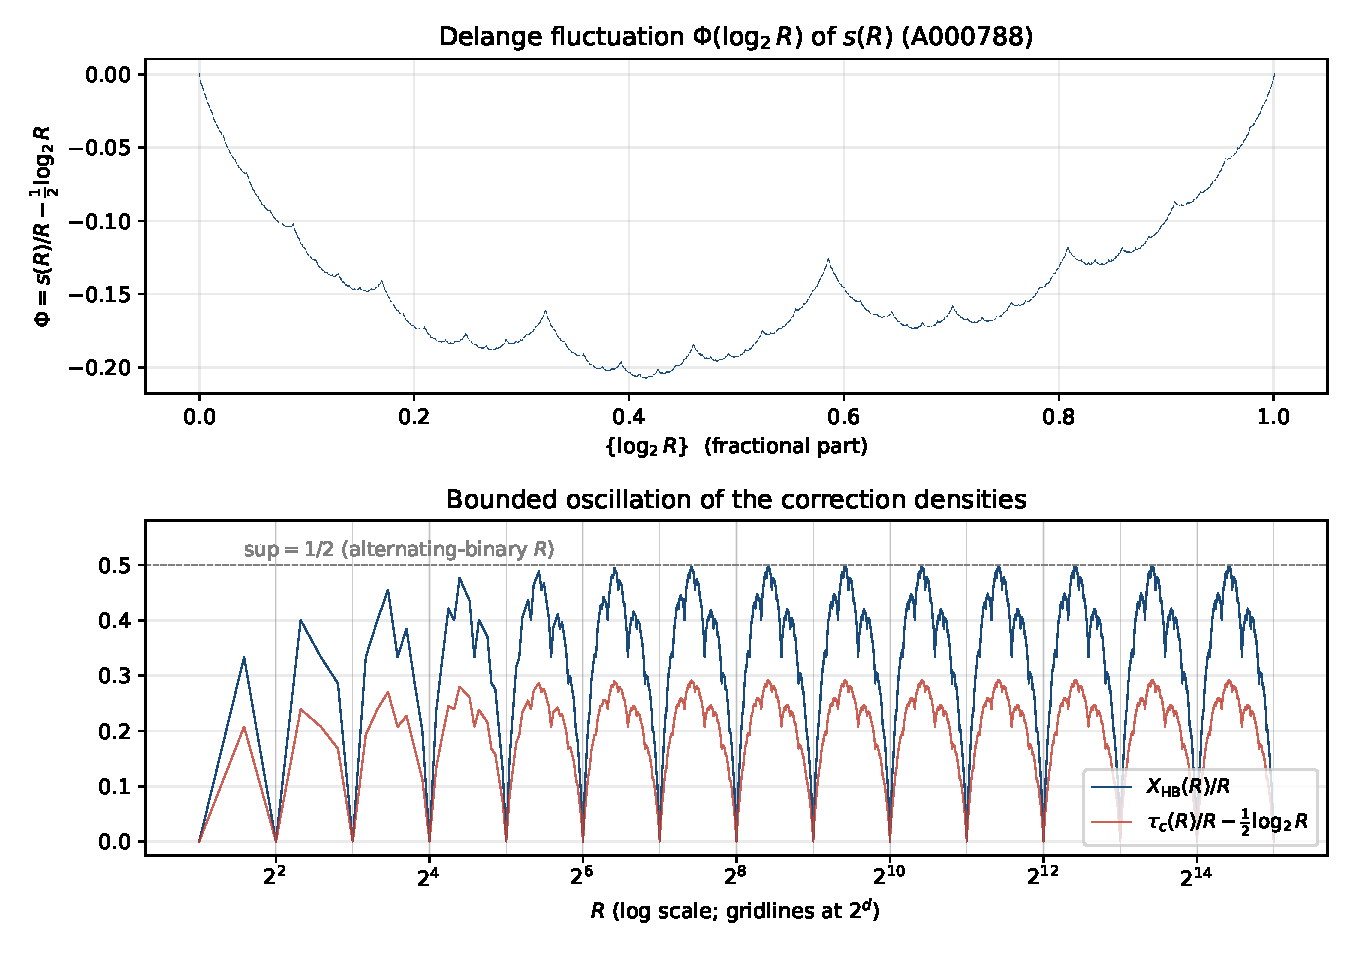
\includegraphics[width=0.92\textwidth]{../assets/out/delange-structure.pdf}
	\caption{Top: the Delange fluctuation $\Phi(\log_2 R)$
		of~\eqref{eq:delange}, computed from $\Eseq(R)$ for
		$256 \le R \le 2^{20}$ and plotted against $\{\log_2 R\}$; the
		self-similar, nowhere-differentiable profile is characteristic of
		radix-$2$ digital sums. Bottom: the centered correction density
		$\Cconst(R)/R - \tfrac{1}{2}\log_2 R$ and the cross-collision density
		$X(\mathrm{HB}_R)/R$ of Corollary~\ref{cor:densities} for
		$2 \le R \le 2^{15}$; both are bounded oscillations in $\log_2 R$,
		vanishing at every power of two (gridlines). The dashed line marks the
		empirical supremum $1/2$ of the cross-collision density, approached
		along the alternating-binary integers
		$R = \lceil 2^{d+1}/3 \rceil$ (e.g.\ $R = 43691 =
			(1010101010101011)_2$ attains $X/R > 0.49998$).}
	\label{fig:delange}
\end{figure}

\begin{remark}[Extremal densities]\label{rem:extremal}
	Numerically, $\sup_R X(\mathrm{HB}_R)/R = \tfrac{1}{2}$ for all sampled
	$R < 2^{16}$ (Figure~\ref{fig:delange}), approached along the
	alternating-binary integers $R = \lceil 2^{d+1}/3\rceil$, which are the
	classical extremizers of the Delange fluctuation; we record this as
	numerical evidence rather than a proven exact supremum, since we have
	not derived it from the Trollope--Delange expansion. The
	graph-theoretic reading is pleasing: the Hamming ball's shielding
	$4$-cycles appear, in this numerical range, to never exceed one per two
	vertices; the largest observed densities occur along the
	alternating-binary integers described above, and they disappear entirely when the ball
	closes into a full subcube.
\end{remark}

\begin{remark}[Relation to the Asymptotic Penalty]\label{rem:penalty-analogy}
	Corollary~\ref{cor:densities} quantifies exactly the $O_R(1)$ terms of
	Theorem~\ref{them:penalty}: in the boundary
	formula~\eqref{eq:extraconnectivity}, the dimension scaling contributes
	the exact linear term in $(n-k)$, while the correction density
	$\Cconst(R)/R$ splits, per~\eqref{eq:C-density}, into a logarithmic trend
	$\tfrac{1}{2}\log_2 R$ plus the bounded oscillation $\Psi(u) -
	\Phi(\log_2 R)$ that carries its entire remaining $R$-dependence.
	Readers
	familiar with analytic
	combinatorics~\cite{wilf2006generatingfunctionology} may recognize the
	division of labor: as in singularity analysis, where a dominant pole
	dictates growth and the remaining analytic part contributes bounded
	corrections, the identity of Theorem~\ref{them:penalty} separates the
	dominant $\Delta D \cdot (n-k)$ term from a topology-dependent constant
	--- though here the separation is an exact finite identity, proved
	directly in the discrete domain, rather than an asymptotic extraction.
\end{remark}
